\chapter{Implémentation  en Spark/Scala} \label{application:spark}

\section{Introduction}

Les fonctionnalités de Spark sont accessibles avec les  APIs en Scala, Java et Python. Nous avons choisi l'utilisation de l'API en Scala parce que Scala est le langage natif de Spark. De plus, Scala est interopérable avec Java. 

Ce chapitre  décrit  l'implémentation de l'outil de détection en utilisant le framework Spark, décrit dans la section \ref{apache-spark}, en utilisant l'API Scala (voir la présentation de Scala dans \ref{scala-presentation}). 
%L'outil implémenté est décrit dans le chapitre \ref{chap:algorith-detection}. 


%[!] Avec Spark, on travaille sur des collections d'objets, sur lesquelles on applique des traitements. Dans une application écrite en Spark, nous avons besoin des classes modélisant les objets tout au long de l'analyse de données, appelées \textit{case class}. De plus, nous avons besoin de définir les fonctions à appliquer  sur ces objets. Nous avons décrit les différentes \textit{case class} conçues pour traiter les objets traceroutes, dans l'annexe \ref{application:spark}, en vue de tracer l'évolution des RTTs différentiels des liens au cours du temps. 

\section{La programmation fonctionnelle et Big Data}
\subsection{Les apports de la programmation fonctionnelle}

\paragraph{Fonctions d'ordre supérieur.} ou  higher-order functions en anglais. Dans un langage, si une fonction est traitée comme first-class value, elle est considérée comme fonction d'ordre supérieur \cite{DBLP:journals/csur/Hudak89}.  

\begin{tcolorbox}
	\textbf{First-class functions}: ou fonctions de première classe dans un langage de programmation sont des fonctions qui peuvent être stockées dans des structures de données, peuvent être passées comme arguments aux fonctions et être retournées comme résultats.
\end{tcolorbox}
\paragraph{Structures de données immuables.} Un objet est immuable est celui qu'on ne peut pas changer son état après sa création. 

\paragraph{Stateless.} Une fonction est dite ayant effet de bord, \textit{side effect} en anglais, quand cette fonction modifie une variable en dehors de son environnement local. Par exemple, les fonctions qui modifient l'état d'une variable passé à cette fonction par référence.

\subsection{La programmation fonctionnelle au service du Big Data }

Quand il s'agit des traitements appliqués sur des données massives dépassant la capacité d'une seule machine, la distribution de ces traitements sur plus d'une machine  est nécessaire. La programmation fonctionnelle peut apporter des facilités aux projets Big Data. On distingue deux sous-catégories de langages de programmation fonctionnelle. Des langages qui sont purement fonctionnels et les autres hybrides.


La programmation fonctionnelle offre de nombreux avantages dans un contexte Big Data. 
L'absence d'effet de bord pour les fonction est un élément clé pour faciliter la parallélisation des traitements appliqués sur des volumes importants de données. Cela permet aussi de mieux gérer les opérations concurrentielles. 
La manipulations des structures de données immuables permet d'écrire un code lisible grâce au nombre réduit de dépendances sur ces structures. De plus, les structures de données immuables facilitent la parallélisation, car elles supportent seulement le mode lecture-seule.
\section{Implémentation}
\subsection{Description de l'environnement}
%Spark est destiné aux traitements distribués sur un cluster de machines, toutefois,n
La création d'une application Spark/Scala passe par les étapes suivantes:
\begin{itemize}
	\item gérer les dépendances nécessaires au fonctionnement de l'application avec le fichier de modèle objet du projet (POM);
	\item écrire l'application dans Scala;
	\item générer le fichier JAR de l'application;
	 \item  exécuter l'application en soumettant cette dernière au cluster. 
\end{itemize}

Dans l'implémentation proposée, nous avons utilisé le mode local de Spark, intitulé \textit{Standalone}. 
Le code source, qui traduit l'ensemble des traitements, est organisé dans une archive de type JAR.
En ce qui concerne  l'automatisation et la gestion du fichier JAR, nous avons utilisé l'outil \textit{Maven}\footnote{\url{https://maven.apache.org/}, consultée le $09/04/2019$.}.
% Les traitements de données sont organisés dans le fichier JAR.


\subsection{Brève présentation  de l'implémentation}

Un programme Spark implique un ensemble d'éléments. La première chose à faire est de configurer le programme Spark.
%et ce à travers  un objet \textit{SparkConf}. Ce dernier contient les informations sur l'application. 
Ensuite, nous utilisons la composante Spark SQL   du Spark Unified Stack (voir la section \ref{Spark Uniffied-Stack}) pour lire les traceroutes présents dans des fichiers d'entrée. Cela permet de créer un Dataset d'objet Traceroute.  Nous convertissons ensuite un Dataset en un RDD afin d'appliquer différentes transformations aboutissant à l'identification des anomalies dans les délais des liens.

\subsection{Création d'une application Spark/Scala}

\paragraph{Gestion des dépendances}~

Le fichier POM permettant de gérer les dépendances est disponible sur GitHub\footnote{\url{https://github.com/hayatbellafkih/SparkSalacaTraceroutesAnalysis/blob/master/rttDelaysSparkScala/pom.xml}, consultée le $23/04/2019$.}. Ces dépendances concernent les composantes de Spark comme spark-core, spark-mllib, spark-sql. De plus, il y a les dépendances permettant de gérer les fichiers de type JSON.


\paragraph{Notation relatives au langage Scala}~

Nous présentons  des notations   propres au langage Scala, elles sont utilisées dans quelques Listings. c'est une liste non exhaustive, elle est utilisée pour comprendre les morceaux de code introduits tout au long de ce chapitre.\\
\textbf{\textit{case class}}: créer une case classe.\\
\textit{\textbf{Seq}}: créer une séquence, équivalent à une liste. Par exemple Seq[String] représente le type d'une liste dont ses éléments sont de type String.  \\
\textbf{\textit{Dataset}}:  est une collection distribuée de données. \\
\textit{\textbf{map}}: permet de transformer le contenu d'une liste en appelant une fonction sur chaque élément de la liste, elle renvoi une liste transformée. \\
\textit{\textbf{Option}} : représente une valeur optionnelle.  \\
\textit{\textbf{groupBy}}: groupBy est une fonction utile pour regrouper les éléments d'une liste ayant une clé en commun.
%Sa définition est : def groupBy[K](f : (A) => K) : Map[K, This] 
\\
\textbf{\textit{List}}: crée une liste d'un type donné. La liste \textit{l\_1} de deux chaînes de caractères est créée comme suit:
\begin{lstlisting}[language=scala,firstnumber=1,label={lst:case-class-hop}, basicstyle = \footnotesize,escapechar=|,numbers=left,
stepnumber=1]
l_1: List[Int] = List("aa", "bb")
\end{lstlisting} 
\noindent \textbf{\textit{filter}} : cette fonction permet de filtrer les éléments d'une collection pour créer une nouvelle collection contenant uniquement les éléments de la collection   vérifiant une condition. Prenons un  exemple : 
\begin{lstlisting}[language=scala,firstnumber=1, basicstyle = \footnotesize,escapechar=|,numbers=left,
stepnumber=1]
//créer une liste d'entier entre 1 et 10, l_2 vaut List(1, 2, 3, 4, 5, 6, 7, 8, 9)
val l_2 = List.range(1, 10)   
// filter les éléments de l_2 afin de ne garder que ceux paires, evens vaut List(2, 4, 6, 8)
val evens = l_2.filter(_ % 2 == 0)  
\end{lstlisting}


\paragraph{Paramètres de l'analyse}~
Afin de tracer l'évolution du délai des liens, nous avons besoin des fichiers stockant les  traceroutes  dans  des objets JSON\footnote{Voir la liste des traceroutes utilisés dans l'exemple illustratif disponible sur GitHub \url{https://github.com/hayatbellafkih/SparkSalacaTraceroutesAnalysis/blob/master/rttDelaysSparkScala/src/main/resources/test/result_modified.json}, consultée le $23/04/2019$.}, la date du début de l'analyse (p. ex. $ 1517961600 $), la date de fin (p. ex. $ 1518134400 $) et enfin la durée d'une période (p. ex. $3600$s). En ce qui concerne les fichiers de données, ils sont stockés localement et le chemin vers ces derniers est configuré dans un fichier de configuration.

\paragraph{Configuration d'une application  Spark}~

Une application Spark nécessite l'ajustement de quelques paramètres, qu'il s'agisse d'une application qui tourne en mode local ou bien en mode cluster. 
 On peut ajuster ces paramètres selon trois possibilités. La première possibilité est à travers l'objet \textit{SparkConf} comme illustré dans l'exemple du Listing \ref{lst:label}, où nous donnons un nom à l'application Spark (ligne \ref{line:app-name}) et nous précisons l'URL du cluster (ligne \ref{line:app-thread}). 

\begin{lstlisting}[language=scala,firstnumber=1, caption={Exemple de configuration avec SparkConf},label={lst:label}, basicstyle = \footnotesize,escapechar=|,numbers=left,
stepnumber=1,numberstyle=\scriptsize]
//imports
import org.apache.spark.SparkConf

// Spark configuration : create configuration
val conf = new SparkConf().setAppName("Link delay analysis") |\label{line:app-name}|
                          .setMaster("local"),  |\label{line:app-thread}|
\end{lstlisting}

Nous pouvons passer certains paramètres au moment de la soumission de l'application au cluster.  Un exemple de ces paramètres est illustré dans le Listing \ref{lst:submit}. Enfin, quelques paramètres peuvent être lus depuis le fichier de configuration  \textit{conf/spark-defaults.conf}\footnote{Plus de détails relatifs à la configuration sont disponibles sur \url{https://spark.apache.org/docs/latest/configuration.html}, consultée le $14/04/2019$.}. 
%Certains paramètres peuvent être précisés 

%en ligne de commande ou bien dans le fichier de configuration \footnote{Plus de détails sont disponibles.}. 
%La configuration de l'application s'effectue à travers un . Il existe un nombre de  paramètres à  ajuster comme le nombre de threads à utiliser au cas où l'application Spark s'exécute en mode local.




\paragraph{Point d'entrée vers les fonctionnalités de Spark}~

Le point d'entrée vers les fonctionnalités de Spark se fait par la création du  \textit{SparkContext}. 
Néanmoins, il existe d'autres points d'entrée qui sont plus spécifiques aux composantes du \textit{Spark Unified Stack}. Par exemple,  \textit{SparkSession}  est le point d'entrée vers Spark SQL, \textit{StreamingContext} est le point d'entrée vers Spark Streaming, etc.
Dans notre cas, nous avons utilisé \textit{SparkSession} pour lire les traceroutes en tant que liste d'objets.



\paragraph{Lecture de données}~

L'outil de détection proposé par R. Fontugne et al. n'exploite qu'une partie des données d'une réponse traceroute\footnote{Un exemple d'une réponse  traceroute  est donné dans l'annexe \ref{exemple-traceroute}.}.
En particulier, on peut utiliser Spark SQL pour  ne lire que les données qui nous intéressent, c'est un des avantages du principe du \textit{Schema-On-Read} décrit dans la section \ref{sec:schema-read-write}. 

Chaque réponse traceroute est structurée dans un objet JSON dans une seule ligne. Afin de lire chaque ligne, nous avons créé la classe Traceroute, cette dernière  a pour objectif de faire l'association entre l'objet JSON  et un objet Traceroute de sorte à encapsuler les données d'un objet JSON. La classe \textit{Traceroute} reprend le nom de la destination de la requête traceroute (\textit{dst\_name}), l'adresse IP de la sonde effectuant la requête traceroute (\textit{from}), l'identifiant de cette sonde (\textit{prb\_id}), le temps de la requête (\textit{timestamp}) et enfin la liste des sauts (\textit{Seq[Hop]}). La classe Traceroute est définie en Scala comme montre le Listing \ref{lst:case-class-Traceroute}.


\begin{lstlisting}[language=scala,firstnumber=1, caption={Définition de la  classe Traceroute},label={lst:case-class-Traceroute}, basicstyle = \footnotesize,escapechar=|,numbers=left,
stepnumber=1]
case class Traceroute(
	dst_name:  String,
	from:      String,
	prb_id:    BigInt,
	msm_id:    BigInt,
	timestamp: BigInt,
	result:    Seq[Hop])
\end{lstlisting}

Un saut  représente un des routeurs parcourus avant d'atteindre la destination finale. Nous modélisons un saut  par la classe \textit{Hop} (voir le Listing \ref{lst:case-class-hop}). Un saut  est défini par son rang (\textit{hop}), ce dernier indique l'ordre du saut en question. Etant donné que la sonde reçoit au moins trois  signaux pour chaque saut. Un saut est donc défini par une liste de signaux (\textit{Seq[Signal]}).
\begin{lstlisting}[language=scala,firstnumber=1, caption={Définition de la  classe Hop},label={lst:case-class-hop}, basicstyle = \footnotesize,escapechar=|,numbers=left,
stepnumber=1]
case class Hop(
	var result: Seq[Signal],
	hop:        Int)
\end{lstlisting}

Un signal (\textit{Signal}) est émis par  un routeur  dont l'adresse IP est \textit{from}. Le temps nécessaire à la réception du signal par la source est   \textit{rtt}. Enfin, \textit{x} est un indicateur de la validité du signal car il se peut que la sonde ne reçoive pas une réponse d'un ou de plusieurs routeurs. Si le signal est valide, \textit{x} est une chaîne vide. Dans le cas d'un signal invalide, \textit{x} vaut "*". Nous précisons qu'un signal est invalide quand la sonde ne reçoit pas une réponse après le temps \textit{tiemout}. Afin d'adapter un saut aussi dans le cas de l'absence des détails du signal, les attributs \textit{rtt}, \textit{x}  et \textit{from} sont définis comme étant optionnels.  
Un signal est modélisé par la classe Signal (voir le Listing \ref{lst:case-class-signal}). 

\begin{lstlisting}[language=scala,firstnumber=1, caption={Définition de la  classe Signal}, label={lst:case-class-signal}, basicstyle = \footnotesize,escapechar=|,numbers=left,
stepnumber=1]
case class Signal(
	rtt:  Option[Double],
	x:    Option[String],
	from: Option[String])
\end{lstlisting}

Nous avons défini  la classe \textit{Traceroute} qui nous permet de lire les données. Pour ce faire, nous utilisons l'objet \textit{spark} de type \textit{SparkSession} créé précédemment. En particulier, nous faisons appel à   la fonction \textit{read()} via ce dernier. Nous spécifions à \textit{read()} le schéma de lecture à travers la classe Traceroute, le chemin vers les fichiers de données (\textit{dataPath}) et comment  les données  sont structurées (\textit{json}). 

\begin{lstlisting}[language=scala,firstnumber=1, caption={La lecture des données traceroutes},label={lst:mapping}, basicstyle = \footnotesize,escapechar=|,numbers=left,
stepnumber=1]
val rawTraceroutes = spark.read
	.schema(Encoders.product[Traceroute].schema)
	.json(dataPath)
	.as[Traceroute]
import spark.implicits._ |\label{lst:implicits}|
 \end{lstlisting}

Nous obtenons la liste des traceroutes dans la variable \textit{rawTraceroutes}. Ce dernier est un Dataset d'objets  Traceroute.
La correspondance entre un enregistrement traceroute JSON et une instance de Traceroute se base sur les noms des attributs dans JSON.
Nous notons que la réussite de la correspondance ne nécessite pas l'association de tous les attributs de l'objet JSON. C'est un des avantages du principe \textit{schema on read}.  Si par exemple, nous définissons des attributs dans la classe Traceroute et que ces attributs ne font pas partie des attributs de l'objet JSON, aucune erreur ne sera survenue.  
La ligne \ref{lst:implicits} du Listing \ref{lst:mapping}  est nécessaire  pour pouvoir utiliser  l'API du Spark, précisément,  les fonctionnalités relatives DataSets et DataFrames. L'appel à la ligne \ref{lst:implicits} du Listing \ref{lst:mapping} ne peut pas être fait sans avoir une instance du \textit{SparkContext}. Dans notre cas, nous avons défini une instance de \textit{SparkSession}, et une instance  de \textit{SparkContext} est fournie, par défaut,  avec cette dernière.


% A , nous appelons certaines fonctionnalités nécessaires à la lecture des données. Il est important de noter que Apache Spark adopte ce qu'on appelle \textit{lazy evaluation}; %(voir la section \ref{lazy-evaluation}). Ainsi,
 %l'évaluation des différentes transformations ne s'effectuent qu'au moment du déclenchement d'une action sur le résultat de cette transformation.

\paragraph{Trouver les périodes de l'analyse}~

Dès à présent, la liste des traceroutes est prête à toute transformation de la phase I (voir la phase I dans la section \ref{processus-de-detection}). 
Tout d'abord, nous devons trouver les périodes entre la date de début et la date de fin (étape \textit{FindBins} (I.1)). 
Cette étape est illustrée par la fonction \textit{generateDateSample}  dans le Listing \ref{lst:findbins};  
 nous construisons les tuples de périodes afin de faciliter le test d'appartenance d'un traceroute, un tuple est formé par le début de la période (\textit{start}),  \textit{start+timewindow}, nous prenons \textit{timewindow} comme étant  équivalent à une heure.


\begin{lstlisting}[language=scala,firstnumber=1, caption={Etape FindBins (I.1)},label={lst:findbins}, basicstyle = \small,escapechar=|,numbers=left,
stepnumber=1]
//Generate the start of all  bins : between start date and end date espaced by the timewindow
val rangeDates = generateDateSample(start, end, timewindow)

// Find the start and the end of each bin
val rangeDatesTimewindows = rangeDates.map(f => (f, f + timewindow))
\end{lstlisting}

A la fin de cette étape, toutes les périodes sont déterminées. Nous passons à l'étape du groupement des traceroutes, disponibles à l'analyse, par période (étape I.2).

\paragraph{Groupement des traceroutes}~

L'objectif de cette étape est de grouper les traceroutes capturés par période. 
Dans l'implémentation du travail de référence\cite{DBLP:journals/corr/FontugneAPB16}, les données sont organisées dans des collections MongoDB (voir la section \ref{subsubsection:mongodb}), le groupement des traceroutes par période se base sur la structuration des noms des collections\footnote{Voir la section \ref{mongodb-impleme}.}. Pour une période donnée, seules les collections concernées  seront interrogées. 
 


\subparagraph{MongoDB}
Nous résumons dans la Figure \ref{fig:read-data-from-mongodb} le groupement  tel qu'il est présenté dans le travail de référence.  
Selon la période en question, nous interrogeons la collection  adéquate.

%A chaque période, les traceroutes sont sélectionnés de la base de données MongoDB en se basant sur les noms des collections. 
\begin{figure}[h]
	\centering
	
	\captionsetup{justification=centering}
	\resizebox{10cm}{6cm}{
	% Graphic for TeX using PGF
% Title: /home/hayat/RipeAtlasTraceroutesAnalysis/2019/Rapport_Mai/illustrations/read-data-from-mongodb.dia
% Creator: Dia v0.97+git
% CreationDate: Thu May  9 00:13:02 2019
% For: hayat
% \usepackage{tikz}
% The following commands are not supported in PSTricks at present
% We define them conditionally, so when they are implemented,
% this pgf file will use them.
\ifx\du\undefined
  \newlength{\du}
\fi
\setlength{\du}{15\unitlength}
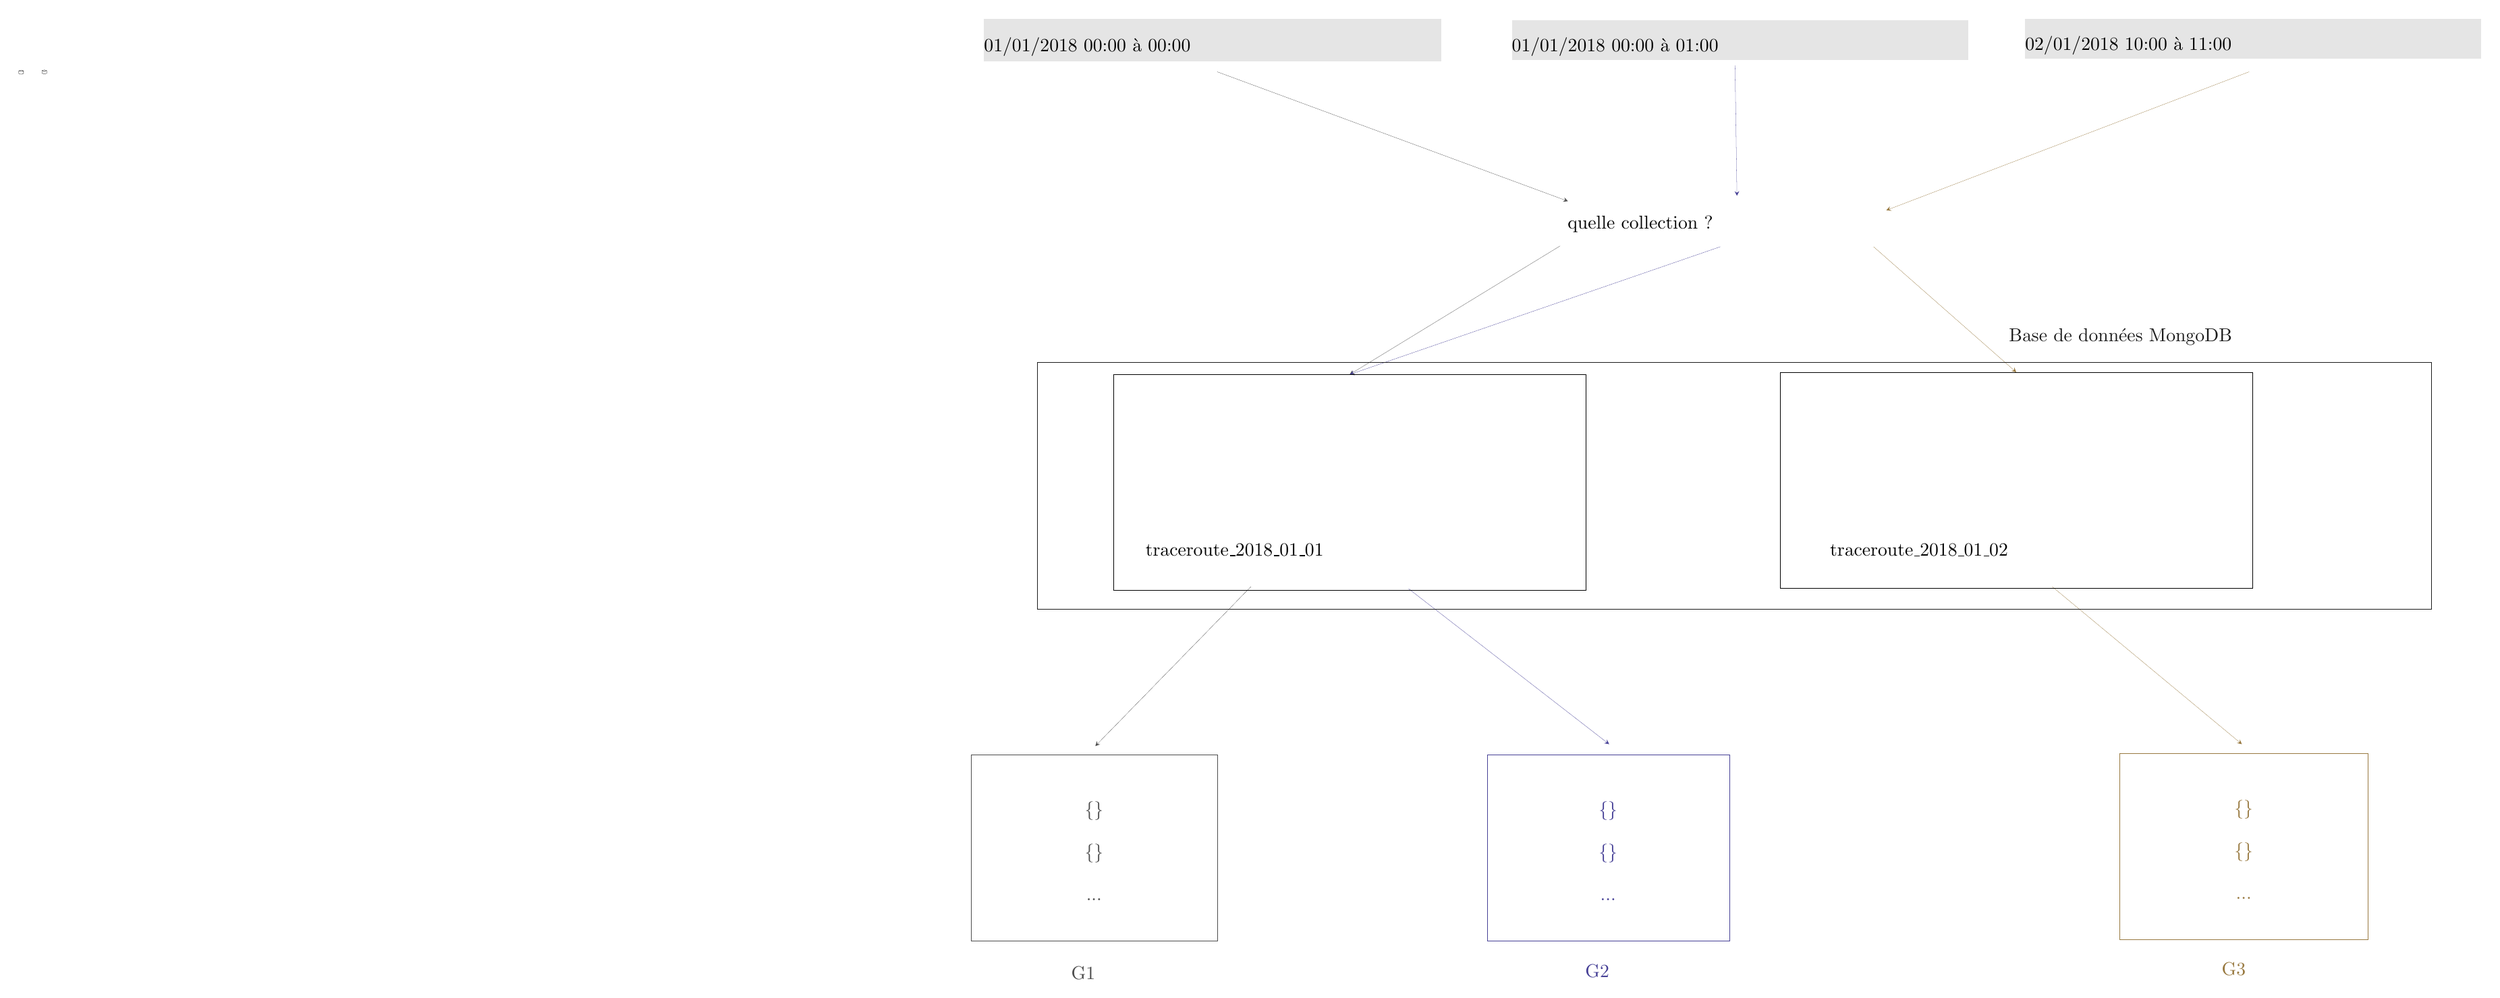
\begin{tikzpicture}[even odd rule]
\pgftransformxscale{1.000000}
\pgftransformyscale{-1.000000}
\definecolor{dialinecolor}{rgb}{0.000000, 0.000000, 0.000000}
\pgfsetstrokecolor{dialinecolor}
\pgfsetstrokeopacity{1.000000}
\definecolor{diafillcolor}{rgb}{1.000000, 1.000000, 1.000000}
\pgfsetfillcolor{diafillcolor}
\pgfsetfillopacity{1.000000}
% setfont left to latex
\definecolor{dialinecolor}{rgb}{0.000000, 0.000000, 0.000000}
\pgfsetstrokecolor{dialinecolor}
\pgfsetstrokeopacity{1.000000}
\definecolor{diafillcolor}{rgb}{0.000000, 0.000000, 0.000000}
\pgfsetfillcolor{diafillcolor}
\pgfsetfillopacity{1.000000}
\node[anchor=base west,inner sep=0pt,outer sep=0pt,color=dialinecolor] at (22.068100\du,9.377600\du){traceroute\_2018\_01\_01};
\pgfsetlinewidth{0.100000\du}
\pgfsetdash{}{0pt}
\pgfsetbuttcap
\pgfsetmiterjoin
\pgfsetlinewidth{0.100000\du}
\pgfsetbuttcap
\pgfsetmiterjoin
\pgfsetdash{}{0pt}
\definecolor{diafillcolor}{rgb}{1.000000, 1.000000, 1.000000}
\pgfsetfillcolor{diafillcolor}
\pgfsetfillopacity{1.000000}
\definecolor{dialinecolor}{rgb}{0.000000, 0.000000, 0.000000}
\pgfsetstrokecolor{dialinecolor}
\pgfsetstrokeopacity{1.000000}
\pgfpathmoveto{\pgfpoint{24.421700\du}{6.810327\du}}
\pgfpathcurveto{\pgfpoint{24.931700\du}{6.535327\du}}{\pgfpoint{25.186700\du}{6.443660\du}}{\pgfpoint{25.696700\du}{6.443660\du}}
\pgfpathcurveto{\pgfpoint{26.206700\du}{6.443660\du}}{\pgfpoint{26.461700\du}{6.535327\du}}{\pgfpoint{26.971700\du}{6.810327\du}}
\pgfpathlineto{\pgfpoint{26.971700\du}{8.276993\du}}
\pgfpathcurveto{\pgfpoint{26.461700\du}{8.551993\du}}{\pgfpoint{26.206700\du}{8.643660\du}}{\pgfpoint{25.696700\du}{8.643660\du}}
\pgfpathcurveto{\pgfpoint{25.186700\du}{8.643660\du}}{\pgfpoint{24.931700\du}{8.551993\du}}{\pgfpoint{24.421700\du}{8.276993\du}}
\pgfpathlineto{\pgfpoint{24.421700\du}{6.810327\du}}
\pgfpathclose
\pgfusepath{fill,stroke}
\pgfsetbuttcap
\pgfsetmiterjoin
\pgfsetdash{}{0pt}
\definecolor{dialinecolor}{rgb}{0.000000, 0.000000, 0.000000}
\pgfsetstrokecolor{dialinecolor}
\pgfsetstrokeopacity{1.000000}
\pgfpathmoveto{\pgfpoint{24.421700\du}{6.810327\du}}
\pgfpathcurveto{\pgfpoint{24.931700\du}{7.085327\du}}{\pgfpoint{25.186700\du}{7.176993\du}}{\pgfpoint{25.696700\du}{7.176993\du}}
\pgfpathcurveto{\pgfpoint{26.206700\du}{7.176993\du}}{\pgfpoint{26.461700\du}{7.085327\du}}{\pgfpoint{26.971700\du}{6.810327\du}}
\pgfusepath{stroke}
% setfont left to latex
\definecolor{dialinecolor}{rgb}{0.000000, 0.000000, 0.000000}
\pgfsetstrokecolor{dialinecolor}
\pgfsetstrokeopacity{1.000000}
\definecolor{diafillcolor}{rgb}{0.000000, 0.000000, 0.000000}
\pgfsetfillcolor{diafillcolor}
\pgfsetfillopacity{1.000000}
\node[anchor=base,inner sep=0pt, outer sep=0pt,color=dialinecolor] at (25.696700\du,7.926993\du){};
% setfont left to latex
\definecolor{dialinecolor}{rgb}{0.101961, 0.101961, 0.101961}
\pgfsetstrokecolor{dialinecolor}
\pgfsetstrokeopacity{1.000000}
\definecolor{diafillcolor}{rgb}{0.101961, 0.101961, 0.101961}
\pgfsetfillcolor{diafillcolor}
\pgfsetfillopacity{1.000000}
\node[anchor=base west,inner sep=0pt,outer sep=0pt,color=dialinecolor] at (38.318500\du,5.336120\du){Base de données MongoDB};
\definecolor{diafillcolor}{rgb}{0.898039, 0.898039, 0.898039}
\pgfsetfillcolor{diafillcolor}
\pgfsetfillopacity{1.000000}
\fill (19.027100\du,-0.736483\du)--(27.628287\du,-0.736483\du)--(27.628287\du,0.067079\du)--(19.027100\du,0.067079\du)--cycle;
% setfont left to latex
\definecolor{dialinecolor}{rgb}{0.000000, 0.000000, 0.000000}
\pgfsetstrokecolor{dialinecolor}
\pgfsetstrokeopacity{1.000000}
\definecolor{diafillcolor}{rgb}{0.000000, 0.000000, 0.000000}
\pgfsetfillcolor{diafillcolor}
\pgfsetfillopacity{1.000000}
\node[anchor=base west,inner sep=0pt,outer sep=0pt,color=dialinecolor] at (19.027100\du,-0.122796\du){01/01/2018 00:00 à 00:00 };
\pgfsetlinewidth{0.100000\du}
\pgfsetdash{}{0pt}
\pgfsetbuttcap
{
\definecolor{diafillcolor}{rgb}{0.301961, 0.301961, 0.301961}
\pgfsetfillcolor{diafillcolor}
\pgfsetfillopacity{1.000000}
% was here!!!
\pgfsetarrowsend{stealth}
\definecolor{dialinecolor}{rgb}{0.301961, 0.301961, 0.301961}
\pgfsetstrokecolor{dialinecolor}
\pgfsetstrokeopacity{1.000000}
\draw (23.412700\du,0.257138\du)--(30.015800\du,2.694520\du);
}
\pgfsetlinewidth{0.100000\du}
\pgfsetdash{}{0pt}
\pgfsetbuttcap
{
\definecolor{diafillcolor}{rgb}{0.301961, 0.301961, 0.301961}
\pgfsetfillcolor{diafillcolor}
\pgfsetfillopacity{1.000000}
% was here!!!
\pgfsetarrowsend{stealth}
\definecolor{dialinecolor}{rgb}{0.301961, 0.301961, 0.301961}
\pgfsetstrokecolor{dialinecolor}
\pgfsetstrokeopacity{1.000000}
\draw (24.049000\du,9.954590\du)--(21.120500\du,12.956300\du);
}
\pgfsetlinewidth{0.100000\du}
\pgfsetdash{}{0pt}
\pgfsetmiterjoin
{\pgfsetcornersarced{\pgfpoint{0.000000\du}{0.000000\du}}\definecolor{diafillcolor}{rgb}{1.000000, 1.000000, 1.000000}
\pgfsetfillcolor{diafillcolor}
\pgfsetfillopacity{1.000000}
\fill (18.779600\du,13.122500\du)--(18.779600\du,16.622500\du)--(23.412688\du,16.622500\du)--(23.412688\du,13.122500\du)--cycle;
}{\pgfsetcornersarced{\pgfpoint{0.000000\du}{0.000000\du}}\definecolor{dialinecolor}{rgb}{0.301961, 0.301961, 0.301961}
\pgfsetstrokecolor{dialinecolor}
\pgfsetstrokeopacity{1.000000}
\draw (18.779600\du,13.122500\du)--(18.779600\du,16.622500\du)--(23.412688\du,16.622500\du)--(23.412688\du,13.122500\du)--cycle;
}% setfont left to latex
\definecolor{dialinecolor}{rgb}{0.301961, 0.301961, 0.301961}
\pgfsetstrokecolor{dialinecolor}
\pgfsetstrokeopacity{1.000000}
\definecolor{diafillcolor}{rgb}{0.301961, 0.301961, 0.301961}
\pgfsetfillcolor{diafillcolor}
\pgfsetfillopacity{1.000000}
\node[anchor=base,inner sep=0pt, outer sep=0pt,color=dialinecolor] at (21.096144\du,14.267500\du){\{\}};
% setfont left to latex
\definecolor{dialinecolor}{rgb}{0.301961, 0.301961, 0.301961}
\pgfsetstrokecolor{dialinecolor}
\pgfsetstrokeopacity{1.000000}
\definecolor{diafillcolor}{rgb}{0.301961, 0.301961, 0.301961}
\pgfsetfillcolor{diafillcolor}
\pgfsetfillopacity{1.000000}
\node[anchor=base,inner sep=0pt, outer sep=0pt,color=dialinecolor] at (21.096144\du,15.067500\du){\{\}};
% setfont left to latex
\definecolor{dialinecolor}{rgb}{0.301961, 0.301961, 0.301961}
\pgfsetstrokecolor{dialinecolor}
\pgfsetstrokeopacity{1.000000}
\definecolor{diafillcolor}{rgb}{0.301961, 0.301961, 0.301961}
\pgfsetfillcolor{diafillcolor}
\pgfsetfillopacity{1.000000}
\node[anchor=base,inner sep=0pt, outer sep=0pt,color=dialinecolor] at (21.096144\du,15.867500\du){...};
% setfont left to latex
\definecolor{dialinecolor}{rgb}{0.000000, 0.000000, 0.000000}
\pgfsetstrokecolor{dialinecolor}
\pgfsetstrokeopacity{1.000000}
\definecolor{diafillcolor}{rgb}{0.000000, 0.000000, 0.000000}
\pgfsetfillcolor{diafillcolor}
\pgfsetfillopacity{1.000000}
\node[anchor=base west,inner sep=0pt,outer sep=0pt,color=dialinecolor] at (21.096200\du,14.872500\du){};
% setfont left to latex
\definecolor{dialinecolor}{rgb}{0.000000, 0.000000, 0.000000}
\pgfsetstrokecolor{dialinecolor}
\pgfsetstrokeopacity{1.000000}
\definecolor{diafillcolor}{rgb}{0.000000, 0.000000, 0.000000}
\pgfsetfillcolor{diafillcolor}
\pgfsetfillopacity{1.000000}
\node[anchor=base west,inner sep=0pt,outer sep=0pt,color=dialinecolor] at (34.949900\du,9.379580\du){traceroute\_2018\_01\_02};
\pgfsetlinewidth{0.100000\du}
\pgfsetdash{}{0pt}
\pgfsetbuttcap
\pgfsetmiterjoin
\pgfsetlinewidth{0.100000\du}
\pgfsetbuttcap
\pgfsetmiterjoin
\pgfsetdash{}{0pt}
\definecolor{diafillcolor}{rgb}{1.000000, 1.000000, 1.000000}
\pgfsetfillcolor{diafillcolor}
\pgfsetfillopacity{1.000000}
\definecolor{dialinecolor}{rgb}{0.000000, 0.000000, 0.000000}
\pgfsetstrokecolor{dialinecolor}
\pgfsetstrokeopacity{1.000000}
\pgfpathmoveto{\pgfpoint{36.864200\du}{6.702487\du}}
\pgfpathcurveto{\pgfpoint{37.374200\du}{6.427487\du}}{\pgfpoint{37.629200\du}{6.335820\du}}{\pgfpoint{38.139200\du}{6.335820\du}}
\pgfpathcurveto{\pgfpoint{38.649200\du}{6.335820\du}}{\pgfpoint{38.904200\du}{6.427487\du}}{\pgfpoint{39.414200\du}{6.702487\du}}
\pgfpathlineto{\pgfpoint{39.414200\du}{8.169153\du}}
\pgfpathcurveto{\pgfpoint{38.904200\du}{8.444153\du}}{\pgfpoint{38.649200\du}{8.535820\du}}{\pgfpoint{38.139200\du}{8.535820\du}}
\pgfpathcurveto{\pgfpoint{37.629200\du}{8.535820\du}}{\pgfpoint{37.374200\du}{8.444153\du}}{\pgfpoint{36.864200\du}{8.169153\du}}
\pgfpathlineto{\pgfpoint{36.864200\du}{6.702487\du}}
\pgfpathclose
\pgfusepath{fill,stroke}
\pgfsetbuttcap
\pgfsetmiterjoin
\pgfsetdash{}{0pt}
\definecolor{dialinecolor}{rgb}{0.000000, 0.000000, 0.000000}
\pgfsetstrokecolor{dialinecolor}
\pgfsetstrokeopacity{1.000000}
\pgfpathmoveto{\pgfpoint{36.864200\du}{6.702487\du}}
\pgfpathcurveto{\pgfpoint{37.374200\du}{6.977487\du}}{\pgfpoint{37.629200\du}{7.069153\du}}{\pgfpoint{38.139200\du}{7.069153\du}}
\pgfpathcurveto{\pgfpoint{38.649200\du}{7.069153\du}}{\pgfpoint{38.904200\du}{6.977487\du}}{\pgfpoint{39.414200\du}{6.702487\du}}
\pgfusepath{stroke}
% setfont left to latex
\definecolor{dialinecolor}{rgb}{0.000000, 0.000000, 0.000000}
\pgfsetstrokecolor{dialinecolor}
\pgfsetstrokeopacity{1.000000}
\definecolor{diafillcolor}{rgb}{0.000000, 0.000000, 0.000000}
\pgfsetfillcolor{diafillcolor}
\pgfsetfillopacity{1.000000}
\node[anchor=base,inner sep=0pt, outer sep=0pt,color=dialinecolor] at (38.139200\du,7.819153\du){};
\definecolor{diafillcolor}{rgb}{0.898039, 0.898039, 0.898039}
\pgfsetfillcolor{diafillcolor}
\pgfsetfillopacity{1.000000}
\fill (28.962000\du,-0.713531\du)--(37.544500\du,-0.713531\du)--(37.544500\du,0.033969\du)--(28.962000\du,0.033969\du)--cycle;
% setfont left to latex
\definecolor{dialinecolor}{rgb}{0.000000, 0.000000, 0.000000}
\pgfsetstrokecolor{dialinecolor}
\pgfsetstrokeopacity{1.000000}
\definecolor{diafillcolor}{rgb}{0.000000, 0.000000, 0.000000}
\pgfsetfillcolor{diafillcolor}
\pgfsetfillopacity{1.000000}
\node[anchor=base west,inner sep=0pt,outer sep=0pt,color=dialinecolor] at (28.962000\du,-0.118531\du){01/01/2018 00:00 à 01:00 };
% setfont left to latex
\definecolor{dialinecolor}{rgb}{0.000000, 0.000000, 0.000000}
\pgfsetstrokecolor{dialinecolor}
\pgfsetstrokeopacity{1.000000}
\definecolor{diafillcolor}{rgb}{0.000000, 0.000000, 0.000000}
\pgfsetfillcolor{diafillcolor}
\pgfsetfillopacity{1.000000}
\node[anchor=base west,inner sep=0pt,outer sep=0pt,color=dialinecolor] at (30.012100\du,3.214930\du){quelle collection ?};
\pgfsetlinewidth{0.100000\du}
\pgfsetdash{}{0pt}
\pgfsetbuttcap
{
\definecolor{diafillcolor}{rgb}{0.274510, 0.250980, 0.588235}
\pgfsetfillcolor{diafillcolor}
\pgfsetfillopacity{1.000000}
% was here!!!
\pgfsetarrowsend{stealth}
\definecolor{dialinecolor}{rgb}{0.274510, 0.250980, 0.588235}
\pgfsetstrokecolor{dialinecolor}
\pgfsetstrokeopacity{1.000000}
\draw (33.160300\du,0.140000\du)--(33.196900\du,2.592620\du);
}
\pgfsetlinewidth{0.100000\du}
\pgfsetdash{}{0pt}
\pgfsetbuttcap
{
\definecolor{diafillcolor}{rgb}{0.274510, 0.250980, 0.588235}
\pgfsetfillcolor{diafillcolor}
\pgfsetfillopacity{1.000000}
% was here!!!
\pgfsetarrowsend{stealth}
\definecolor{dialinecolor}{rgb}{0.274510, 0.250980, 0.588235}
\pgfsetstrokecolor{dialinecolor}
\pgfsetstrokeopacity{1.000000}
\draw (27.014100\du,9.991200\du)--(30.791300\du,12.920900\du);
}
\pgfsetlinewidth{0.100000\du}
\pgfsetdash{}{0pt}
\pgfsetmiterjoin
{\pgfsetcornersarced{\pgfpoint{0.000000\du}{0.000000\du}}\definecolor{diafillcolor}{rgb}{1.000000, 1.000000, 1.000000}
\pgfsetfillcolor{diafillcolor}
\pgfsetfillopacity{1.000000}
\fill (28.492000\du,13.124500\du)--(28.492000\du,16.624500\du)--(33.050493\du,16.624500\du)--(33.050493\du,13.124500\du)--cycle;
}{\pgfsetcornersarced{\pgfpoint{0.000000\du}{0.000000\du}}\definecolor{dialinecolor}{rgb}{0.274510, 0.250980, 0.588235}
\pgfsetstrokecolor{dialinecolor}
\pgfsetstrokeopacity{1.000000}
\draw (28.492000\du,13.124500\du)--(28.492000\du,16.624500\du)--(33.050493\du,16.624500\du)--(33.050493\du,13.124500\du)--cycle;
}% setfont left to latex
\definecolor{dialinecolor}{rgb}{0.274510, 0.250980, 0.588235}
\pgfsetstrokecolor{dialinecolor}
\pgfsetstrokeopacity{1.000000}
\definecolor{diafillcolor}{rgb}{0.274510, 0.250980, 0.588235}
\pgfsetfillcolor{diafillcolor}
\pgfsetfillopacity{1.000000}
\node[anchor=base,inner sep=0pt, outer sep=0pt,color=dialinecolor] at (30.771246\du,14.269500\du){\{\}};
% setfont left to latex
\definecolor{dialinecolor}{rgb}{0.274510, 0.250980, 0.588235}
\pgfsetstrokecolor{dialinecolor}
\pgfsetstrokeopacity{1.000000}
\definecolor{diafillcolor}{rgb}{0.274510, 0.250980, 0.588235}
\pgfsetfillcolor{diafillcolor}
\pgfsetfillopacity{1.000000}
\node[anchor=base,inner sep=0pt, outer sep=0pt,color=dialinecolor] at (30.771246\du,15.069500\du){\{\}};
% setfont left to latex
\definecolor{dialinecolor}{rgb}{0.274510, 0.250980, 0.588235}
\pgfsetstrokecolor{dialinecolor}
\pgfsetstrokeopacity{1.000000}
\definecolor{diafillcolor}{rgb}{0.274510, 0.250980, 0.588235}
\pgfsetfillcolor{diafillcolor}
\pgfsetfillopacity{1.000000}
\node[anchor=base,inner sep=0pt, outer sep=0pt,color=dialinecolor] at (30.771246\du,15.869500\du){...};
% setfont left to latex
\definecolor{dialinecolor}{rgb}{0.000000, 0.000000, 0.000000}
\pgfsetstrokecolor{dialinecolor}
\pgfsetstrokeopacity{1.000000}
\definecolor{diafillcolor}{rgb}{0.000000, 0.000000, 0.000000}
\pgfsetfillcolor{diafillcolor}
\pgfsetfillopacity{1.000000}
\node[anchor=base west,inner sep=0pt,outer sep=0pt,color=dialinecolor] at (30.771200\du,14.874500\du){};
\pgfsetlinewidth{0.100000\du}
\pgfsetdash{}{0pt}
\pgfsetbuttcap
{
\definecolor{diafillcolor}{rgb}{0.301961, 0.301961, 0.301961}
\pgfsetfillcolor{diafillcolor}
\pgfsetfillopacity{1.000000}
% was here!!!
\pgfsetarrowsend{stealth}
\definecolor{dialinecolor}{rgb}{0.301961, 0.301961, 0.301961}
\pgfsetstrokecolor{dialinecolor}
\pgfsetstrokeopacity{1.000000}
\draw (29.869400\du,3.536470\du)--(25.907300\du,5.958560\du);
}
\pgfsetlinewidth{0.100000\du}
\pgfsetdash{}{0pt}
\pgfsetbuttcap
{
\definecolor{diafillcolor}{rgb}{0.274510, 0.250980, 0.588235}
\pgfsetfillcolor{diafillcolor}
\pgfsetfillopacity{1.000000}
% was here!!!
\pgfsetarrowsend{stealth}
\definecolor{dialinecolor}{rgb}{0.274510, 0.250980, 0.588235}
\pgfsetstrokecolor{dialinecolor}
\pgfsetstrokeopacity{1.000000}
\draw (32.884800\du,3.551780\du)--(25.907300\du,5.958560\du);
}
\definecolor{diafillcolor}{rgb}{0.898039, 0.898039, 0.898039}
\pgfsetfillcolor{diafillcolor}
\pgfsetfillopacity{1.000000}
\fill (38.621400\du,-0.743276\du)--(47.203900\du,-0.743276\du)--(47.203900\du,0.004224\du)--(38.621400\du,0.004224\du)--cycle;
% setfont left to latex
\definecolor{dialinecolor}{rgb}{0.000000, 0.000000, 0.000000}
\pgfsetstrokecolor{dialinecolor}
\pgfsetstrokeopacity{1.000000}
\definecolor{diafillcolor}{rgb}{0.000000, 0.000000, 0.000000}
\pgfsetfillcolor{diafillcolor}
\pgfsetfillopacity{1.000000}
\node[anchor=base west,inner sep=0pt,outer sep=0pt,color=dialinecolor] at (38.621400\du,-0.148276\du){02/01/2018 10:00 à 11:00 };
\pgfsetlinewidth{0.100000\du}
\pgfsetdash{}{0pt}
\pgfsetbuttcap
{
\definecolor{diafillcolor}{rgb}{0.596078, 0.474510, 0.250980}
\pgfsetfillcolor{diafillcolor}
\pgfsetfillopacity{1.000000}
% was here!!!
\pgfsetarrowsend{stealth}
\definecolor{dialinecolor}{rgb}{0.596078, 0.474510, 0.250980}
\pgfsetstrokecolor{dialinecolor}
\pgfsetstrokeopacity{1.000000}
\draw (42.837400\du,0.257138\du)--(36.007800\du,2.865390\du);
}
\pgfsetlinewidth{0.100000\du}
\pgfsetdash{}{0pt}
\pgfsetmiterjoin
{\pgfsetcornersarced{\pgfpoint{0.000000\du}{0.000000\du}}\definecolor{diafillcolor}{rgb}{1.000000, 1.000000, 1.000000}
\pgfsetfillcolor{diafillcolor}
\pgfsetfillopacity{1.000000}
\fill (40.400700\du,13.097400\du)--(40.400700\du,16.597400\du)--(45.070700\du,16.597400\du)--(45.070700\du,13.097400\du)--cycle;
}{\pgfsetcornersarced{\pgfpoint{0.000000\du}{0.000000\du}}\definecolor{dialinecolor}{rgb}{0.596078, 0.474510, 0.250980}
\pgfsetstrokecolor{dialinecolor}
\pgfsetstrokeopacity{1.000000}
\draw (40.400700\du,13.097400\du)--(40.400700\du,16.597400\du)--(45.070700\du,16.597400\du)--(45.070700\du,13.097400\du)--cycle;
}% setfont left to latex
\definecolor{dialinecolor}{rgb}{0.596078, 0.474510, 0.250980}
\pgfsetstrokecolor{dialinecolor}
\pgfsetstrokeopacity{1.000000}
\definecolor{diafillcolor}{rgb}{0.596078, 0.474510, 0.250980}
\pgfsetfillcolor{diafillcolor}
\pgfsetfillopacity{1.000000}
\node[anchor=base,inner sep=0pt, outer sep=0pt,color=dialinecolor] at (42.735700\du,14.242400\du){\{\}};
% setfont left to latex
\definecolor{dialinecolor}{rgb}{0.596078, 0.474510, 0.250980}
\pgfsetstrokecolor{dialinecolor}
\pgfsetstrokeopacity{1.000000}
\definecolor{diafillcolor}{rgb}{0.596078, 0.474510, 0.250980}
\pgfsetfillcolor{diafillcolor}
\pgfsetfillopacity{1.000000}
\node[anchor=base,inner sep=0pt, outer sep=0pt,color=dialinecolor] at (42.735700\du,15.042400\du){\{\}};
% setfont left to latex
\definecolor{dialinecolor}{rgb}{0.596078, 0.474510, 0.250980}
\pgfsetstrokecolor{dialinecolor}
\pgfsetstrokeopacity{1.000000}
\definecolor{diafillcolor}{rgb}{0.596078, 0.474510, 0.250980}
\pgfsetfillcolor{diafillcolor}
\pgfsetfillopacity{1.000000}
\node[anchor=base,inner sep=0pt, outer sep=0pt,color=dialinecolor] at (42.735700\du,15.842400\du){...};
% setfont left to latex
\definecolor{dialinecolor}{rgb}{0.000000, 0.000000, 0.000000}
\pgfsetstrokecolor{dialinecolor}
\pgfsetstrokeopacity{1.000000}
\definecolor{diafillcolor}{rgb}{0.000000, 0.000000, 0.000000}
\pgfsetfillcolor{diafillcolor}
\pgfsetfillopacity{1.000000}
\node[anchor=base west,inner sep=0pt,outer sep=0pt,color=dialinecolor] at (42.735700\du,14.847400\du){};
\pgfsetlinewidth{0.100000\du}
\pgfsetdash{}{0pt}
\pgfsetbuttcap
{
\definecolor{diafillcolor}{rgb}{0.596078, 0.474510, 0.250980}
\pgfsetfillcolor{diafillcolor}
\pgfsetfillopacity{1.000000}
% was here!!!
\pgfsetarrowsend{stealth}
\definecolor{dialinecolor}{rgb}{0.596078, 0.474510, 0.250980}
\pgfsetstrokecolor{dialinecolor}
\pgfsetstrokeopacity{1.000000}
\draw (35.767600\du,3.551780\du)--(38.453500\du,5.915880\du);
}
\pgfsetlinewidth{0.100000\du}
\pgfsetdash{}{0pt}
\pgfsetbuttcap
{
\definecolor{diafillcolor}{rgb}{0.596078, 0.474510, 0.250980}
\pgfsetfillcolor{diafillcolor}
\pgfsetfillopacity{1.000000}
% was here!!!
\pgfsetarrowsend{stealth}
\definecolor{dialinecolor}{rgb}{0.596078, 0.474510, 0.250980}
\pgfsetstrokecolor{dialinecolor}
\pgfsetstrokeopacity{1.000000}
\draw (39.130700\du,9.954590\du)--(42.700100\du,12.920900\du);
}
\pgfsetlinewidth{0.100000\du}
\pgfsetdash{}{0pt}
\pgfsetmiterjoin
\pgfsetbuttcap
{\pgfsetcornersarced{\pgfpoint{0.000000\du}{0.000000\du}}\definecolor{dialinecolor}{rgb}{0.000000, 0.000000, 0.000000}
\pgfsetstrokecolor{dialinecolor}
\pgfsetstrokeopacity{1.000000}
\draw (34.005900\du,5.915880\du)--(34.005900\du,9.979179\du)--(42.901230\du,9.979179\du)--(42.901230\du,5.915880\du)--cycle;
}\pgfsetlinewidth{0.100000\du}
\pgfsetdash{}{0pt}
\pgfsetmiterjoin
\pgfsetbuttcap
{\pgfsetcornersarced{\pgfpoint{0.000000\du}{0.000000\du}}\definecolor{dialinecolor}{rgb}{0.000000, 0.000000, 0.000000}
\pgfsetstrokecolor{dialinecolor}
\pgfsetstrokeopacity{1.000000}
\draw (21.459600\du,5.958560\du)--(21.459600\du,10.021859\du)--(30.354930\du,10.021859\du)--(30.354930\du,5.958560\du)--cycle;
}\pgfsetlinewidth{0.100000\du}
\pgfsetdash{{\pgflinewidth}{0.200000\du}}{0cm}
\pgfsetmiterjoin
\pgfsetbuttcap
{\pgfsetcornersarced{\pgfpoint{0.000000\du}{0.000000\du}}\definecolor{dialinecolor}{rgb}{0.101961, 0.101961, 0.101961}
\pgfsetstrokecolor{dialinecolor}
\pgfsetstrokeopacity{1.000000}
\draw (20.022300\du,5.725990\du)--(20.022300\du,10.381298\du)--(46.269317\du,10.381298\du)--(46.269317\du,5.725990\du)--cycle;
}% setfont left to latex
\definecolor{dialinecolor}{rgb}{0.301961, 0.301961, 0.301961}
\pgfsetstrokecolor{dialinecolor}
\pgfsetstrokeopacity{1.000000}
\definecolor{diafillcolor}{rgb}{0.301961, 0.301961, 0.301961}
\pgfsetfillcolor{diafillcolor}
\pgfsetfillopacity{1.000000}
\node[anchor=base west,inner sep=0pt,outer sep=0pt,color=dialinecolor] at (20.667200\du,17.348100\du){G1};
% setfont left to latex
\definecolor{dialinecolor}{rgb}{0.274510, 0.250980, 0.588235}
\pgfsetstrokecolor{dialinecolor}
\pgfsetstrokeopacity{1.000000}
\definecolor{diafillcolor}{rgb}{0.274510, 0.250980, 0.588235}
\pgfsetfillcolor{diafillcolor}
\pgfsetfillopacity{1.000000}
\node[anchor=base west,inner sep=0pt,outer sep=0pt,color=dialinecolor] at (30.341800\du,17.318500\du){G2};
% setfont left to latex
\definecolor{dialinecolor}{rgb}{0.596078, 0.474510, 0.250980}
\pgfsetstrokecolor{dialinecolor}
\pgfsetstrokeopacity{1.000000}
\definecolor{diafillcolor}{rgb}{0.596078, 0.474510, 0.250980}
\pgfsetfillcolor{diafillcolor}
\pgfsetfillopacity{1.000000}
\node[anchor=base west,inner sep=0pt,outer sep=0pt,color=dialinecolor] at (42.322600\du,17.279500\du){G3};
\end{tikzpicture}

}
	\caption{Groupement des traceroutes avec MongoDB}
	\label{fig:read-data-from-mongodb}
\end{figure}

Nous illustrons ce groupement avec un pseudo-code décrit par l'algorithme \ref{group-traceroutesmongodb}.

\begin{algorithm}[H]
	\caption{Groupement des traceroutes dans le cas de MongoDB}
	\label{group-traceroutesmongodb}
	\begin{algorithmic}
		%\For{$traceroute$ $\in$ $rawTraceroutes$} 
		%\State \texttt{Attribuer $traceroute$ à }
		
		\For{$period$ $\in$ $rangeDatesTimewindows$} 
		\State $collection$ $\gets$ \texttt{Trouver la collection incluant $period$}
		\State \texttt{$rawTraceroutes$ $\gets$   les traceroutes stockés dans  $collection$ et enregistrés durant $period$}
		
     ...	\Comment{Traitements appliqués sur l'ensemble de traceroutes}
		%\State \texttt{Vérifier si  $traceroute$ appartient à  $period$}
		\EndFor
		%\EndFor
	\end{algorithmic}
\end{algorithm}

Cette manière de grouper les traceroutes ne prend pas en considération le cas où
il faut chercher les traceroutes dans plus d'une collection.

\subparagraph{Spark/Scala} En ce qui concerne l'implémentation en Spark/Scala,
 nous avons groupé les traceroutes autrement. 
 %en partant de ces derniers. 
 Les traceroutes sont organisés dans des fichiers reprenant des traceroutes d'une heure, d'une journée ou d'une toute autre période.  Peu importe le nombre de ces fichiers, Spark lit tout ce qui est disponible dans le chemin \textit{dataPath}. 
 Notons que le  parcours de tous les fichiers à chaque  période est coûteux en terme de performance.
  C'est pourquoi nous avons attribué les traceroutes aux périodes. Dans ce cas, les fichiers de données sont lus une seule fois. C'est ce que nous résumons dans l'algorithme \ref{group-data-sparkscala}. Les lignes entre \ref{initate-list} et \ref{finloop1} de l'algorithme \ref{group-data-sparkscala} permettent d'associer chaque traceroute à une période faisant partie de la période de l'analyse. La ligne  \ref{groupby} permet de grouper les traceroutes par période; il s'agit de grouper les traceroutes ayant la même période. L'objectif des lignes entre \ref{begin-groupby} et \ref{end-groupby}  de l'algorithme \ref{group-data-sparkscala} est d'appliquer les traitements sur les groupes de traceroutes, cependant, elles ne sont pas détaillés dans cet algorithme. 
  
  %Seuls les traceroutes qui font partie de la période de l'analyse à un traceroute, on teste toutes les périodes jusqu'à trouver la période adéquate.

\begin{algorithm}[H]
	\caption{Groupement des traceroutes en Spark}
	\label{group-data-sparkscala}
	\begin{algorithmic}[1]
    \State $ traceroutePerPeriod $  $\gets$ [] \label{initate-list}
	\For{$traceroute$ $\in$ $rawTraceroutes$} 
	%\State \texttt{Attribuer $traceroute$ à }
	
		\For{$period$ $\in$ $rangeDatesTimewindows$} 
			\State \texttt{Vérifier si  $traceroute$ appartient à  $period$}
		\EndFor
		\State \texttt{$ traceroutePerPeriod $.append(($ traceroute $, $period$))}
	\EndFor  \label{finloop1}
	\State \texttt{$ traceroutesPerPeriods $ $\gets$$ traceroutePerPeriods $.groupBy($period$)} \label{groupby}
	\For{$element$ $\in$ $ traceroutesPerPeriods $}\label{begin-groupby}
	\State ... \Comment{Traitements appliqués sur l'ensemble de traceroutes}
	\EndFor \label{end-groupby}

\end{algorithmic}
\end{algorithm}

En Spark/Scala, nous avons chargé les traceroutes disponibles à l'analyse sur un RDD. Ce dernier crée des partitions de données, sensées être manipulées sur différentes machines si Spark est lancé sur un cluster de machine. Afin de créer les groupes de traceroutes, nous vérifions l'appartenance de chaque traceroute à une des périodes considérées.

\begin{lstlisting}[language=scala,firstnumber=1, caption={},label={lst:groupalltraceroutes}, basicstyle = \small,escapechar=|,numbers=left,
stepnumber=1]
//Group each traceroute by the bin that they belong in 
// If one traceroute does not belongs in any bin, then by default it belongs to the bin 0
val tracerouteAndPeriodRdd = rawTraceroutes.rdd.map(traceroute => TracerouteWithTimewindow(traceroute, findTimeWindowOfTraceroute(traceroute, rangeDatesTimewindows)))|\label{line:groupTraceroutes}|
\end{lstlisting}

Avec la ligne \ref{line:groupTraceroutes} dans le Listing \ref{lst:groupalltraceroutes} :

\begin{itemize}
	\item nous transformons  \textit{rawTraceroutes}  en un RDD;
	\item pour chaque objet Traceroute, nous appliquons le traitement du groupement en utilisant la méthode \textit{findTimeWindowOfTraceroute}. Cette dernière prend en paramètre le traceroute et les périodes possibles dont ce dernier peut y appartient et elle renvoie la période adéquate;
	\item nous passons d'un RDD de type \textit{Traceroute} à un RDD de type \textit{TracerouteWithPeriod}.
\end{itemize}

La  classe \textit{TracerouteWithPeriod}, définie dans le Listing \ref{lst:TracerouteWithTimewindow}, permet de représenter un traceroute avec sa période dans une seule entité. 
\begin{lstlisting}[language=scala,firstnumber=1, caption={Définition de la classe TracerouteWithPeriod },label={lst:TracerouteWithTimewindow}, basicstyle = \footnotesize,escapechar=|,numbers=left,
stepnumber=1]
case class TracerouteWithPeriod(
	traceroute: Traceroute,
	period:     Int)
\end{lstlisting}

\subparagraph{Elimination des traceroutes qui n'appartiennent pas à l'analyse}~

Il se peut qu'un traceroute ne fait pas partie de la période de l'analyse. Ce sont les objets de type \textit{TracerouteWithPeriod}  ayant  \textit{period} de valeur $0$ et période = 0 si traceroute.timestamp n'appartient à aucune des période. C'est pourquoi nous filtrons ces traceroutes, comme  illustre le Listing  \ref{lst:filterTracerouteWithTimewindow}.

\begin{lstlisting}[language=scala,firstnumber=1, caption={Elimination des traceroutes non concernés par l'analyse },label={lst:filterTracerouteWithTimewindow}, basicstyle = \footnotesize,escapechar=|,numbers=left,
stepnumber=1]
val onlyConcernedTraceroutes = tracerouteAndPeriodRdd.filter(_.period != 0)
\end{lstlisting}

Après l'élimination des traceroutes non concernés, nous agrégeons ces derniers par période pour construire une liste de type   \textit{TraceroutesPerPeriod} dont sa définition est  donnée dans le Listing \ref{lst:classTraceroutesPerPeriod}. 
L'objectif de cette agrégation est de créer des groupes de traceroutes et y  appliquer les traitements relatifs à la détection. 
Le Listing \ref{lst:agregatePeriodTraceroutes} illustre l'étape de l'agrégation.


\begin{lstlisting}[language=scala,firstnumber=1, caption={Le groupement des traceroutes },label={lst:agregatePeriodTraceroutes}, basicstyle = \footnotesize,escapechar=|,numbers=left,
stepnumber=1]
val groupedTraceroutesByPeriod = onlyConcernedTraceroutes.groupBy(_.period)
val traceroutesPerPeriod = groupedTraceroutesByPeriod.map(f => TraceroutesPerPeriod(f._2.map(f => f.traceroute).toSeq, f._1))
\end{lstlisting}


\begin{lstlisting}[language=scala,firstnumber=1, caption={Définition de la classe TraceroutesPerPeriod },label={lst:classTraceroutesPerPeriod}, basicstyle = \footnotesize,escapechar=|,numbers=left,
stepnumber=1]
case class TraceroutesPerPeriod(
	traceroutes: Seq[Traceroute],
	period:  Int)
\end{lstlisting}

\paragraph{Déduction des liens}~

L'étape qui suit le groupement des traceroutes est la génération des liens. Ainsi, nous générons les différents liens possibles dans chacune des périodes avec le code du Listing \ref{lst:linkInference} :

\begin{lstlisting}[language=scala,firstnumber=1, caption={La classe TracerouteWithPeriod },label={lst:linkInference}, basicstyle = \footnotesize,escapechar=|,numbers=left,
stepnumber=1]
val allLinksRttDiffsPeriods = traceroutesPerPeriod.map(f => linksInference(spark, f))
\end{lstlisting}

La fonction \textit{linksInference} est une abstraction de plusieurs traitements appliqués sur chaque groupe de traceroutes.  Cette fonction renvoie
la liste des liens caractérisés par leurs périodes et RTTs différentiels. Le Listing \ref{lst:DeductionLinks}
illustre les étapes de la déduction des liens par groupe de traceroutes, ces étapes sont les suivantes : 

\begin{enumerate}
	\item élimination des traceroutes échoués;
	\item élimination des sauts non valides;
	\item calcul de la médiane de chaque saut;
	\item lister les liens possibles par traceroute en encapsulant ces derniers dans des objets \textit{DetailedLink};
	\item construction d'une liste reprenant les listes de l'étape $4$.
	\item tri alphanumérique des adresses IP de chaque lien;
	\item groupement des liens ayant les mêmes adresses IP;
	\item création d'un récapitulatif de chaque lien; chaque lien est associé à une liste des RTTs différentiels ainsi que la liste des périodes. La liste des périodes contient la période courante dupliquée en nombre de RTTs différentiels de ce lien durant cette période. 
\end{enumerate}

%Les étapes énumérées ci-dessus sont illustrées par le Listing \ref{lst:DeductionLinks}.

\begin{lstlisting}[language=scala,firstnumber=1, caption={Deduction des liens par groupe de traceroutes},label={lst:DeductionLinks}, basicstyle = \footnotesize,escapechar=|,numbers=left,
stepnumber=1]
 def linksInference(spark: SparkSession, rawtraceroutes: TraceroutesPerPeriod): Seq[ResumedLink] = {
	
	//Filter failed traceroutes ... 
	val notFailedTraceroutes = rawtraceroutes.traceroutes.filter(t => t.result(0).result != null) |\label{notFailedTraceroutes}|
	
	//Remove invalid data  in hops
	val cleanedTraceroutes = notFailedTraceroutes.map(t => removeInvalidSignals(t)) |\label{cleanedTraceroutes}|
	
	//Compute median by hop
	val tracerouteMedianByHop = cleanedTraceroutes.map(t => computeMedianRTTByhop(t)) |\label{tracerouteMedianByHopline}|
	
	//Find links in a traceroute
	import org.apache.spark.mllib.rdd.RDDFunctions._
	val tracerouteLinks = tracerouteMedianByHop.map(t => findLinksAndRttDiffByTraceroute(spark, t)) |\label{tracerouteLinksline}|
	
	//Create a set of DetailedLink objects for every traceroute
	val detailedLinks = tracerouteLinks.map(summarizeLinksTraceroute) |\label{liens-par-périodeline}|
	
	//Flatten the list of lists to have one liste of DetailedLink objects
	val allDetailedLinks = detailedLinks.flatten |\label{allDetailedLinksFlattenline}|
	
	//Sort the links
	val sortAllDetailedLinks = allDetailedLinks.map(l => sortLinks(l)) |\label{sortAllDetailedLinksline}|
	
	//Merge the links from all traceroutes in the current bin
	val mergedLinks = sortAllDetailedLinks.groupBy(_.link) |\label{mergedLinksline}|
	
	//Summarize the link 
	val summarizeLink = mergedLinks.map(f => ResumedLink(f._1, f._2.map(_.probe), f._2.map(_.rttDiff), generateDatesSample(f._2.size, rawtraceroutes.timeWindow)))  |\label{summarizeLinkline}|
	
	summarizeLink.toSeq    
}
\end{lstlisting}


Nous reprenons dans les sections suivantes la définition de fonctions utilisées dans la fonction \textit{linksInference}.

\subparagraph{Elimination des traceroutes échoués} (Ligne \ref{notFailedTraceroutes} dans le Listing \ref{lst:DeductionLinks}) Nous parcourons chaque traceroute de la liste des traceroutes \textit{rawtraceroutes.traceroutes} afin d'éliminer tout traceroute échoué. Dans l'implémentation de l'outil de détection, ils ont constaté que la liste des sauts d'un traceroute échoué contient un seul saut (\textit{t.result(0)}) et la liste des signaux n'existe pas (\textit{t.result(0).result != null}). Avec \textit{t} dénote le traceroute courant dans la liste \textit{rawtraceroutes.traceroutes}. 


\subparagraph{Elimination des sauts non valides} (Ligne \ref{cleanedTraceroutes} dans le Listing \ref{lst:DeductionLinks}) Nous parcourons les traceroutes valides (\textit{notFailedTraceroutes}) et nous appliquons  \textit{removeInvalidSignals} sur chaque traceroute. Cette fonction renvoie un traceroute après avoir appliqué la fonction \textit{checkSignal} sur chaque signal de chaque saut. 

\begin{lstlisting}[language=scala,firstnumber=1, caption={Définition de la méthode removeInvalidSignals},label={lst:removeInvalidSignals}, basicstyle = \footnotesize,escapechar=|,numbers=left,
stepnumber=1]
  def removeInvalidSignals(traceroute: Traceroute): Traceroute = {
	val hops = traceroute.result
	for (hop <- hops) {
		val signals = hop.result
		val tmpSignals = signals.filter(checkSignal(_))
		hop.result = tmpSignals
	}
	traceroute
}
\end{lstlisting}

Le rôle de la fonction \textit{checkSignal}, définie dans le Listing \ref{lst:checkSignal},  est de vérifier chaque signal : si le signal est valide (Ligne \ref{timesout}), si le RTT existe (Ligne \ref{rttnotnone}), si le RTT est positif \label{rttpositif} et enfin si le signal ne provient pas d'une adresse IP privée (Ligne \ref{notprivate}).

\begin{lstlisting}[language=scala,firstnumber=1, caption={Définition de la méthode checkSignal},label={lst:checkSignal}, basicstyle = \footnotesize,escapechar=|,numbers=left,
stepnumber=1]
  def checkSignal(signal: Signal): Boolean = {
	//Check if a signal is not failled
	if (signal.x == "*") |\label{timesout}|
	return false
	// Check if the RTT exist
	else if (signal.rtt == None) |\label{rttnotnone}|
	return false
	else if (signal.rtt.get <= 0) { |\label{rttpositif}|
		return false
	} else if (javatools.Tools.isPrivateIp(signal.from.get)) |\label{notprivate}|
	return false
	else {
		return true
	}
  }
\end{lstlisting}

\subparagraph{Calcul de la médiane de chaque saut} (Ligne \ref{tracerouteMedianByHopline} dans le Listing \ref{lst:DeductionLinks})
Après avoir vérifié les sauts des traceroutes, nous appelons la fonction \textit{computeMedianRTTByhop}  présentée dans le Listing \ref{lst:computeMedianRTTByhopFunction} pour calculer la médiane des RTTs par saut. Dans un premier temps, la fonction \textit{computeMedianRTTByhop} récupère les sauts du traceroute donné en entrée, elle calcule la médiane des RTTs et renvoi un traceroute avec des RTTs agrégés. 

\begin{lstlisting}[language=scala,firstnumber=1, caption={Définition de la fonction computeMedianRTTByhop},label={lst:computeMedianRTTByhopFunction}, basicstyle = \footnotesize,escapechar=|,numbers=left,
stepnumber=1]  
  def computeMedianRTTByhop(traceroute: Traceroute): MedianByHopTraceroute = {
	val hops = traceroute.result
	val procHops = hops.map(f => findMedianFromSignals(f))
	s
	MedianByHopTraceroute(traceroute.dst_name, traceroute.from, traceroute.prb_id, traceroute.msm_id, traceroute.timestamp, procHops)
}
\end{lstlisting}

Le traceroute renvoyé est de type \textit{MedianByHopTraceroute}. Ce dernier est défini dans le Listing \ref{lst:MedianByHopTracerouteclass}. Une instance de la classe \textit{Traceroute} est se diffère  d'une instance de la classe \textit{MedianByHopTraceroute} au niveau de l'attribut \textit{result} qui désigne la liste des sauts.
\begin{lstlisting}[language=scala,firstnumber=1, caption={Définition de la classe MedianByHopTraceroute},label={lst:MedianByHopTracerouteclass}, basicstyle = \footnotesize,escapechar=|,numbers=left,
stepnumber=1] 
case class MedianByHopTraceroute(
	dst_name:  String,
	from:      String,
	prb_id:    BigInt,
	msm_id:    BigInt,
	timestamp: BigInt           = 0,
	result:    Seq[PreparedHop])
\end{lstlisting}

La nouvelle classe qui représente un saut est définie dans le Listing \ref{lst:PreparedHopclass}.
\begin{lstlisting}[language=scala,firstnumber=1, caption={Définition de la classe PreparedHop},label={lst:PreparedHopclass}, basicstyle = \footnotesize,escapechar=|,numbers=left,
stepnumber=1] 
case class PreparedHop(
	var result: Seq[PreparedSignal],
	hop:        Int)
\end{lstlisting}

Dans la nouvelle définition du saut, ce dernier est toujours défini par une liste de signaux, car la sonde peut recevoir les signaux, pour un même saut, depuis différents routeurs. La nouvelle classe représentant un signal est définie dans le Listing \ref{lst:PreparedSignalclass}, où \textit{medianRtt} est la médiane des RTTs en provenance du routeur \textit{from}. 
\begin{lstlisting}[language=scala,firstnumber=1, caption={Définition de la classe PreparedSignal},label={lst:PreparedSignalclass}, basicstyle = \footnotesize,escapechar=|,numbers=left,
stepnumber=1] 
case class PreparedSignal(
	medianRtt: Double,
	from:      String)
\end{lstlisting}

\subparagraph{Enumération des liens possibles par traceroute et leur RTT différentiel} (Ligne \ref{tracerouteLinksline} du Listing \ref{lst:DeductionLinks})  La fonction \textit{findLinksAndRttDiffByTraceroute} prend en paramètre une instance de \textit{MedianByHopTraceroute} et renvoie une instance de \textit{LinksTraceroute}. Les liens sont déduits suivant l'approche décrite dans la Figure \ref{fig:link-inference}. Le rôle de cette méthode est de parcourir les sauts afin de construire les liens possibles. Précisément, c'est la fonction findAllLinks (Ligne \ref{findAllLinksline} du Listing \ref{lst:functionfindLinksAndRttDiffByTraceroute}) qui crée les liens possibles pour tous deux sauts consécutifs et calcule leur RTT différentiel.

\begin{lstlisting}[language=scala,firstnumber=1, caption={Définition de la fonction findLinksAndRttDiffByTraceroute},label={lst:functionfindLinksAndRttDiffByTraceroute}, basicstyle = \footnotesize,escapechar=|,numbers=left,
stepnumber=1] 
  def findLinksAndRttDiffByTraceroute(spark: SparkSession, traceroute: MedianByHopTraceroute): LinksTraceroute = {
	val hops = traceroute.result
	val size = hops.size
	val s = hops.zipWithIndex
	val z = s.map {
		case (element, index) =>
		if (index + 1 < size) {
			findAllLinks(hops(index + 1), element) |\label{findAllLinksline}|
		} else {
			null
		}
	}
	return new LinksTraceroute(traceroute.dst_name, traceroute.from, traceroute.prb_id, traceroute.msm_id, traceroute.timestamp, z.filter(p => p != null).flatten)
}
\end{lstlisting}

 La fonction \textit{findAllLinks}, définie dans le Listing \ref{lst:findAllLinksfunction}, prend deux paramètres de type \textit{PreparedHop} : \textit{nextHop} et \textit{currentHop}. Cette fonction renvoie la liste des liens (\textit{links}) avec leur RTT différentiel. 
 
 \begin{lstlisting}[language=scala,firstnumber=1, caption={Définition de la fonction findAllLinks},label={lst:findAllLinksfunction}, basicstyle = \footnotesize,escapechar=|,numbers=left,
 stepnumber=1] 
  def findAllLinks(nextHop: PreparedHop, currentHop: PreparedHop): Seq[Link] = {
	var links = Seq[Link]()
	
	for (nextRouter <- nextHop.result) {
		for (currentRouter <- currentHop.result) {
			val rttDiff = BigDecimal(nextRouter.medianRtt) - BigDecimal(currentRouter.medianRtt)
			links = links :+ Link(nextRouter.from, currentRouter.from, rttDiff.toDouble)
		}
	}
	return links
}
\end{lstlisting}

Après avoir parcouru les sauts consécutifs du traceroute, nous créons une instance de la classe \textit{LinksTraceroute}. Cette classe reprend la liste des liens au lieu de la liste des sauts avec les autres informations du traceroute. La définition de cette classe est donnée dans le Listing :
\begin{lstlisting}[language=scala,firstnumber=1, caption={Définition de la fonction},label={lst:function}, basicstyle = \footnotesize,escapechar=|,numbers=left,
stepnumber=1] 
case class LinksTraceroute(
	dst_name:  String,
	from:      String,
	prb_id:    BigInt,
	msm_id:    BigInt,
	timestamp: BigInt,
	links:     Seq[Link])
\end{lstlisting}

La classe \textit{Link} modélise un lien et son RTT différentiel (voir le Listing \ref{lst:Linkclass}).
\begin{lstlisting}[language=scala,firstnumber=1, caption={Définition de la classe Link},label={lst:Linkclass}, basicstyle = \footnotesize,escapechar=|,numbers=left,
stepnumber=1] 
case class Link(
	ip1:     String,
	ip2:     String,
	rttDiff: Double)
\end{lstlisting}

\subparagraph{Construction de la liste des liens par période } (Ligne \ref{liens-par-périodeline} du Listing \ref{lst:DeductionLinks})
%	\item lister les liens possibles par traceroute en encapsulant ces derniers dans des objets \textit{DetailedLink};tracerouteLinks
A cette étape, nous souhaitons réorganiser les liens précédemment énumérés par traceroute. L'objectif de cette réorganisation est de passer des liens identifiés dans le cadre d'un traceroute (une instance de \textit{LinksTraceroute}) à une liste de liens (plusieurs instances de \textit{DetailedLink}) comme illustre la définition de la fonction summarizeLinksTraceroute dans le Listing \ref{lst:summarizeLinksTraceroutefunction}. 


\begin{lstlisting}[language=scala,firstnumber=1, caption={Définition de la fonction summarizeLinksTraceroute},label={lst:summarizeLinksTraceroutefunction}, basicstyle = \footnotesize,escapechar=|,numbers=left,
stepnumber=1] 
  def summarizeLinksTraceroute(traceroute: LinksTraceroute): Seq[DetailedLink] = {
	val links = traceroute.links
	val summarizedLinks = links.map(f => DetailedLink(f.rttDiff, LinkIPs(f.ip1, f.ip2), traceroute.prb_id))
	summarizedLinks
}
\end{lstlisting}

La classe \textit{DetailedLink}, définie dans le Listing \ref{lst:DetailedLinkclass}, permet  modéliser un seul lien. 
\begin{lstlisting}[language=scala,firstnumber=1, caption={Définition de la classe DetailedLink},label={lst:DetailedLinkclass}, basicstyle = \footnotesize,escapechar=|,numbers=left,
stepnumber=1] 
case class DetailedLink(
	rttDiff:  Double,
	var link: LinkIPs,
	probe:    BigInt)
\end{lstlisting}

La fonction \textit{linksInference} est appliqué sur chaque groupe de traceroutes. Dans ce cas, pour chaque groupe de traceroutes, on associe une liste des liens encapsulés chacun dans une instance de \textit{DetailedLink}. Maintenant que chaque lien reprend l'information de la période pendant laquelle il a été identifié, nous pouvons créer une liste d'instance de \textit{DetailedLink} concernant toutes les périodes. C'est ce que fait la ligne \ref{allDetailedLinksFlattenline} dans la fonction dans le Listing \ref{lst:DeductionLinks}.

\subparagraph{Tri alphanumérique des adresses IP de chaque lien} (Ligne \ref{sortAllDetailedLinksline} dans le Listing \ref{lst:DeductionLinks}). La méthode \textit{sortLinks}, définie dans le Listing \ref{lst:sortLinksfunction}, permet de trier les deux adresses IP du lien donné en paramètre et renvoi un nouveau lien.
\begin{lstlisting}[language=scala,firstnumber=1, caption={Définition de la fonction sortLinks},label={lst:sortLinksfunction}, basicstyle = \footnotesize,escapechar=|,numbers=left,
stepnumber=1] 
def sortLinks(linkToSort: DetailedLink): DetailedLink = {
	val link = Seq(linkToSort.link.ip1, linkToSort.link.ip2)
	val sortedLink = link.sorted
	linkToSort.link = LinkIPs(sortedLink(0), sortedLink(1))
	linkToSort
}
\end{lstlisting}


\subparagraph{Groupement des liens ayant les mêmes adresses IP} (Ligne \ref{mergedLinksline} dans le Listing \ref{lst:DeductionLinks})
Nous regroupons les liens par leurs adresses IP en utilisant la fonction GroupBy de Scala.

\subparagraph{Création d'un récapitulatif de chaque lien} (Ligne \ref{summarizeLinkline} dans le Listing \ref{lst:DeductionLinks})
C'est la dernière étape de la phase de la préparation de données.  L'objectif de cette étape est de regrouper les même lien dans une seule entité, représentée par une instance de la classe \textit{ResumedLink} définie dans le Listing \ref{lst:ResumedLinkClasscase}.
 Cette classe reprend les deux  adresses IP du lien (\textit{link}), la liste des sondes ayant identifié ce lien (\textit{probes}), la liste des RTTs différentiels de ce lien (\textit{rttDiffs}) et enfin les \textit{periods} qui  représentent les périodes  pendant lesquelles les \textit{rttDiffs} ont été identifiés. 


\begin{lstlisting}[language=scala,firstnumber=1, caption={Définition de la classe ResumedLink},label={lst:ResumedLinkClasscase}, basicstyle = \footnotesize,escapechar=|,numbers=left,
stepnumber=1]
case class SummarizedLink(
	link:     LinkIPs,
	probes:   Seq[BigInt],
	rttDiffs: Seq[Double],
	var periods: Seq[Int])
\end{lstlisting}


\paragraph{Caractérisation des liens de toutes les périodes de l'analyse}~

Après avoir traité tous les groupes de traceroutes, nous obtenons un RDD de liste de liens (\textit{RDD[Seq[classes.ResumedLink]]}). Nous devons collecter les résultats des traitements de chacune des partitions de ce RDD afin de passer à la phase II de l'analyse des délais. Dans le cas d'un cluster de machines, il s'agit de la collecte de ces résultats de la part de chaque machine.  
Le code illustrant la collecte des résultats est illustrée par le Listing \ref{lst:rddcollecte}. Autrement dit, le \textit{driver}  reçoit les résultats des traitements appliqués sur les données et effectués par les \textit{workers}\footnote{Voir le principe de la distribution des traitements en Spark dans la section \ref{sparkpresentationsection}.}.

\begin{lstlisting}[language=scala,firstnumber=1, caption={Collecte des résultats intermédiares },label={lst:rddcollecte}, basicstyle = \footnotesize,escapechar=|,numbers=left,
stepnumber=1]
val finalLinksDetailsList = allLinksRttDiffsPeriods.collect().toSeq.flatten
\end{lstlisting}

Après avoir collecté les résultats intermédiaires, nous fusionnons les données des liens en provenance de toutes les périodes. C'est ce que illustre le Listing \ref{lst:rddmergeLinks}. La différence entre cette collecte et la collecte précédente (Ligne \ref{allDetailedLinksFlattenline} dans le Listing \ref{lst:DeductionLinks}), c'est que la première a été faite au niveau d'un \textit{worker}, or, la collecte précédente est fait au niveau du \textit{driver}.

\begin{lstlisting}[language=scala,firstnumber=1, caption={Fusion des liens de toute la période de l'analyse},label={lst:rddmergeLinks}, basicstyle = \footnotesize,escapechar=|,numbers=left,
stepnumber=1]

// Merge all links from all periods
val finalResult = collectedRTTDiff.groupBy(_.link)
val finalRawRttDiff = finalResult.map(f => ResumedLink(
                                            f._1, 
                                            (f._2.map(_.probes)).flatten, 
                                            (f._2.map(_.rttDiffs)).flatten, 
                                            (f._2.map(_.periods)).flatten)
                                     )
\end{lstlisting}

Commentaires  du Listing \ref{lst:rddmergeLinks} :

\noindent \textit{finalResult} est de type Map  : la clé est de type \textit{LinkIPs} et la valeur est de type

\noindent \textit{Seq[classes.SummarizedLink]} (\textit{Map[classes.LinkIPs, Seq[classes.SummarizedLink]]}).

\noindent En parcourons  \textit{finalResult}, l'élément courant parcouru $f$ contient deux partie, vu qu'il appartient à une Map, la première, $ f\_1 $, représente la clé (de type \textit{LinkIPs})  et la deuxième,  $ f\_2 $, représente la valeur (de type  \textit{Seq[classes.SummarizedLink]}).  Ainsi, le rôle de \textit{f.\_2.map(\_.periods)).flatten} est parcourir (via la fonction map) la liste des liens, et de récupérer en particulier la liste des période stockée dans \textit{periods} enfin regrouper toute les période en une seule liste (via flatten).


A cette étape, nous avons une liste de type \textit{ResumedLink} qui concerne  la période entière de l'analyse. 
%Ce dernier est définie dans le Listing \ref{lst:ResumedLinkClasscase}. 

%\begin{lstlisting}[language=scala,firstnumber=1, caption={Définition de la classe ResumedLink},label={lst:ResumedLinkClass}, basicstyle = \footnotesize,escapechar=|,numbers=left,
%stepnumber=1]
%case class ResumedLink(
%	link:     LinkIPs,
%	probes:   Seq[BigInt],
%	rttDiffs: Seq[Double],
%	var bins: Seq[Int])
%\end{lstlisting}


\paragraph{Détection des anomalies}~

Nous présentons dans ce qui suit la phase II de l'analyse des délais. A travers la méthode \textit{listAlarms()} nous analysons un lien et nous identifions les anomalies de ce dernier. Dans le Listing \ref{lst:paralelizeAndDtectAnomalies}, d'abord nous convertissons la liste des liens en un RDD afin de distribuer le traitement de ces liens. Ensuite, nous appliquons la méthode \textit{listAlarms} sur tout lien. 


A la fin de la phase I, nous obtenons une liste des liens de type \textit{Iterable}  

(Iterable[classes.SummarizedLink]). Comme chaque lien peut être traité indépendamment des autres liens, nous créons un RDD à partir de cette liste (Ligne \ref{parallelizefinalRawRttDiff} du Listing \ref{lst:paralelizeAndDtectAnomalies}), ensuite, nous appliquons la méthode sur chaque lien (Ligne \ref{listAlarmscall} du Listing \ref{lst:paralelizeAndDtectAnomalies}).  

\begin{lstlisting}[language=scala,firstnumber=1, caption={Détection des alarmes des liens},label={lst:paralelizeAndDtectAnomalies}, basicstyle = \footnotesize,escapechar=|,numbers=left,
stepnumber=1]
// Create a RDD having the ResumedLink elements from stage I
val finalRawRttDiffRdd = spark.sparkContext.parallelize(finalRawRttDiff.toSeq) |\label{parallelizefinalRawRttDiff}|

// Alarms detection by link
val linkAnalysisResult = finalRawRttDiffRdd.map(p => listAlarms(spark, p, timewindow, rangeDates)) |\label{listAlarmscall}|
\end{lstlisting}

La méthode \textit{listAlarms} est détaillée dans le Listing \ref{lst:findAnalomalies}. Dans cette dernière, nous assurons:


\begin{enumerate}
	\item initialisation des variables : \textit{reference} est l'état référence du lien, \textit{current} est l'état courant du lien, \textit{alarmsValues} est la liste des alarmes qui sont des RTTs différentiels médians, \textit{alarmsDates} est la liste dates correspondantes aux alarmes, \textit{dates} est la liste des dates concernées; ce sont les périodes ayant une distribution des RTTs différentiels de taille plus grande d'un nombre donné.
	\item  génération des périodes; nous générons les périodes correspondantes à au moins une journée;
    \item  en partant des périodes générées, dans leurs ordre chronologique, nous appliquons la méthode \textit{findAlarms()} sur les RTTs différentiels de chaque période;
    \item enfin, nous construisons un objet JSON reprenant les détails du lien. A savoir, leurs périodes, leurs anomalies et leurs dates d'anomalies. 
\end{enumerate}

\begin{lstlisting}[language=scala,firstnumber=1, caption={Définition de la méthode listAlarms},label={lst:findAnalomalies}, basicstyle = \footnotesize,escapechar=|,numbers=left,
stepnumber=1]
  def listAlarms(spark: SparkSession, rawDataLinkFiltred: ResumedLink, timewindow: Int, rangeDates: Seq[Int]): String = {
	// Save the reference state of a link
	var reference = LinkState(Seq(), Seq(), Seq(), Seq())
	
	// Save the current state of a link
	var current = LinkState(Seq(), Seq(), Seq(), Seq())
	
	// Save the RTT differentials anomalies
	var alarmsValues = AlarmsValues()
	
	// Save the dates having delay anomalies
	var alarmsDates = AlarmsDates()
	
	// Save all the dates to draw the evolution 
	var dates = AllDates()
	
	val rawDataLink = rawDataLinkFiltred
	
	/*Regardless of the period specified in the inputs, the evolution is created for one or more days
	* Eg : if the period is only 2 hours, the evolution is created for 24 hours,
	* and the begin date is the begin date given in inputs
	* */
	val start = rawDataLink.bins.min
	val max = rawDataLink.bins.max
	val diferenceDays = (max - start) / 60 / 60 / 24
	val end = start + ((diferenceDays + 1) * 86400)
	
	//Find all the bins in the selected days
	val datesEvolution = start.to(end - timewindow).by(timewindow)
	
	// For each bin, find the data (RTTs differentials) and find alarms
	datesEvolution.foreach(f => findAlarms(spark, f, reference, rawDataLink, current, alarmsDates, alarmsValues, dates))
	
	// create a JSON string to save the results
	implicit val formats = DefaultFormats
	val linkEvolution = LinkEvolution(rawDataLink.link, reference, current, alarmsDates.dates, alarmsValues.medians, dates.dates)
	val linkEvolutionJsonStr = write(linkEvolution)
	linkEvolutionJsonStr
}
\end{lstlisting}

La définition de la fonction \textit{findAlarms} est donnée dans le Listing \ref{lst:findAlarmsFunction}. Cette méthode s'applique sur les données d'un lien,
son objectif  est de comparer l'état courant du lien en question avec la référence suivant les trois cas détaillés dans l'étape II.5 du processus décrit dans la section \ref{processus-de-detection}.


\begin{lstlisting}[language=scala,firstnumber=1, caption={Définition de la méthode findAlarms},label={lst:findAlarmsFunction}, basicstyle = \footnotesize,escapechar=|,numbers=left,
stepnumber=1]
  def findAlarms(spark: SparkSession, date: Int, reference: LinkState, dataPeriod: ResumedLink, current: LinkState, alarmsDates: AlarmsDates, alarmsValues: AlarmsValues, dates: AllDates): Unit = {
	println("Find indices ...")
	val indices = dataPeriod.bins.zipWithIndex.filter(_._1 == date).map(_._2)
	val dist = indices.map(f => dataPeriod.rttDiffs(f))
	
	println("Find RTTs for the current timewindow ...")
	val distSize = dist.size
	
	if (distSize > 3) {
		val tmpDates = dates.dates :+ date
		dates.dates = tmpDates
		
		// Compute the Wilson Score
		val wilsonCi = scoreWilsonScoreCalculator(spark, dist.size).map(f => f * dist.size)
		
		//update the current link state
		updateLinkCurrentState(spark, dist, current, wilsonCi)
		
		//Sort the distribution
		val newDist = dist.sorted
		
		//Get the reference
		val tmpReference = reference
		
		// Case : 1
		if (tmpReference.valueMedian.size < 3) {
			val newReferenceValueMedian = tmpReference.valueMedian :+ current.valueMedian.last
			val newReferenceValueHi = tmpReference.valueHi :+ newDist(javatools.JavaTools.getIntegerPart(wilsonCi(1)))
			val newReferenceValueLow = tmpReference.valueLow :+ newDist(javatools.JavaTools.getIntegerPart(wilsonCi(0)))
			
			reference.valueHi = newReferenceValueHi
			reference.valueLow = newReferenceValueLow
			reference.valueMedian = newReferenceValueMedian
			
		} //Case : 2
		else if (reference.valueMedian.size == 3) {
			
			val newReferenceValueMedian1 = tmpReference.valueMedian :+ medianCalculator(tmpReference.valueMedian)
			val newReferenceValueHi1 = tmpReference.valueHi :+ medianCalculator(tmpReference.valueHi)
			val newReferenceValueLow1 = tmpReference.valueLow :+ medianCalculator(tmpReference.valueLow)
			
			reference.valueHi = newReferenceValueHi1
			reference.valueLow = newReferenceValueLow1
			reference.valueMedian = newReferenceValueMedian1
			
			val newReferenceValueMedian = reference.valueMedian.map(f => reference.valueMedian.last)
			reference.valueMedian = newReferenceValueMedian
			val newReferenceValueHi = reference.valueHi.map(f => reference.valueHi.last)
			reference.valueHi = newReferenceValueHi
			val newReferenceValueLow = reference.valueLow.map(f => reference.valueLow.last)
			reference.valueLow = newReferenceValueLow
		} //Case : 3
		else {
			
			val newReferenceValueMedian2 = tmpReference.valueMedian :+ (0.99 * tmpReference.valueMedian.last + 0.01 * current.valueMedian.last)
			val newReferenceValueHi2 = tmpReference.valueHi :+ (0.99 * tmpReference.valueHi.last + 0.01 * newDist(javatools.JavaTools.getIntegerPart(wilsonCi(1))))
			val newReferenceValueLow2 = tmpReference.valueLow :+ (0.99 * tmpReference.valueLow.last + 0.01 * newDist(javatools.JavaTools.getIntegerPart(wilsonCi(0))))
			reference.valueHi = newReferenceValueHi2
			reference.valueLow = newReferenceValueLow2
			reference.valueMedian = newReferenceValueMedian2
			
			//Anomalies dection : compare the current with the reference
			if ((BigDecimal(current.valueMedian.last) - BigDecimal(current.valueLow.last) > reference.valueHi.last || current.valueMedian.last + current.valueHi.last < reference.valueLow.last) && scala.math.abs(current.valueMedian.last - reference.valueMedian.last) > 1) {
				
				val updateAlarmsDates = alarmsDates.dates :+ date
				alarmsDates.dates = updateAlarmsDates
				
				val updateAlarmsValues = alarmsValues.medians :+ current.valueMedian.last
				alarmsValues.medians = updateAlarmsValues
			}
		}
	}
}
\end{lstlisting}

 Nous résumons le fonctionnement de la méthode \textit{findAlarms} dans les étapes suivantes. Notons que \textit{spark}  est l'objet SparkSession créé au début du programme Spark,  \textit{date} est la période courante, \textit{reference} est l'état référence du lien, \textit{dataPeriod} est la liste des RTTs différentiels de la période  \textit{date}, \textit{current} est l'état courant du lien, \textit{alarmsDates} sont les dates d'alarmes, \textit{alarmsValues} sont les RTTs différentiels médians et \textit{dates} sont les dates où on constate une distribution assez représentable des RTTs différentiels.   
 
 \begin{enumerate}
 	\item trouver les indices,  dans \textit{dataPeriod.bins}, correspondants à la période \textit{date} (\textit{indices});
 	
 	\item trouver les RTTs différentiels, dans \textit{dataPeriod.rttDiffs}, identifiés durant  \textit{date} (\textit{dist});
 	
 	\item la représentativité d'une distribution dépend d'une valeur donnée  (ici $3$), Si la taille de \textit{dist} est supérieure à cette valeur, nous ajoutons \textit{date} à \textit{dates} et nous continuons l'analyse de cette période;
 	\item calculer le score de Wilson, qui fournit deux valeurs, et multiplier ce score par la taille de la distribution;
 	\item calculer l'état courant du lien (\textit{current}), cela inclut la borne inférieure de l'intervalle de confiance, le RTT différentiel médian et la borne supérieure de l'intervalle de confiance;
 	\item  récupérer l'état référence du lien;
 	\item mettre à jour l'état référence du lien \textit{reference} suivant les trois cas;
 	\item  comparer les deux intervalles de confiance s'il s'agit du cas $3$ et mettre à jour \textit{alarmsValues} et \textit{alarmsDates} si une anomalie est identifiée.
 	
 \end{enumerate}



\subsection{Exécution d'une application Spark} Afin de pouvoir exécuter une application Spark, il faut qu'elle soit packagée dans un fichier de type JAR. Ce dernier doit reprendre une classe contenant une méthode \textit{main} et doit reprendre toutes les dépendances nécessaires à l'exécution de l'application.  Enfin, l'application Spark  est soumise avec la commande \textit{bin/spark-submit}. Un exemple d'une soumission est donné dans \ref{lst:submit}.

\begin{lstlisting}[language=bash,firstnumber=1, caption={Exemple de la soumissions d'un traitement sur Spark},label={lst:submit}, basicstyle = \small,escapechar=|,numbers=left,
stepnumber=1]
~$ bin/spark-submit --class ripeatlasanalysis.AnalyseTraceroute     --master local --driver-memory 30G  --conf "spark.network.timeout=10000000" DelayAnalysis-0.0.5-SNAPSHOT-jar-with-dependencies.jar  1517961600  1518134400 3600 
\end{lstlisting}
La commande \textit{bin/spark-submit} prend plusieurs paramètres, nous présentons quelques paramètres utilisés :
\begin{itemize}
	\item \textit{class} est un objet Scala contenant la fonction \textit{main};
	\item  \textit{master} est l'URL du cluster (voir les différents modes dans la section \ref{spark-master-modes});
	\item \textit{driver-memory} est la mémoire dont le processus du driver peut utiliser;
	
	\item  \textit{--conf} "key = value" est une manière de configurer l'application Spark. Dans l'exemple, "spark.network.timeout=10000000", $ 10000000 $ est le temps durant lequel le driver doit recevoir  des mises à jour de la part des différents workers; après ce temps, le worker n'est plus considéré comme actif.
\end{itemize}

\paragraph{Résultats finaux}~

Nous sauvegardons le résultat de l'analyse dans un fichier JSON en vue de toute réutilisation. Un exemple de résultat est illustré dans le Listing \ref{resultLink}.

\begin{lstlisting}[language=json,firstnumber=1, caption={Exemple des résultats de l'analyse d'un lien}, label=resultLink]
{
	"link": {
		"ip1": "185.147.12.31",
		"ip2": "89.105.200.57"
	},
	"reference": {
		"valueMedian": [
		2.991,
		2.991,
		2.991,
		2.991,
		13.67572,
		13.5727878
		],
		"valueHi": [
		4.402,
		4.402,
		4.402,
		4.402,
		15.352609999999999,
		15.243713899999998
		],
		"valueLow": [
		2.394,
		2.394,
		2.394,
		2.394,
		12.83469,
		12.7333531
		],
		"valueMean": []
	},
	"current": {
		"valueMedian": [
		2.991,
		3.081,
		2.9109999999999996,
		823.963,
		1071.463,
		3.3825000000000003
		],
		"valueHi": [
		0.472,
		1.321,
		1.7240000000000004,
		175.5,
		28,
		1.0804999999999998
		],
		"valueLow": [
		10.741,
		0.39,
		0.5169999999999996,
		142.5,
		25,
		0.6815000000000003
		],
		"valueMean": []
	},
	"alarmsDates": [
	1514784200,
	1514787800
	],
	"alarmsValues": [
	1071.463,
	3.3825000000000003
	],
	"dates": [
	1514769800,
	1514773400,
	1514777000,
	1514780600,
	1514784200,
	1514787800
	]
}
\end{lstlisting}
\section{Conclusion}

